\documentclass[oneside, final, 12pt]{article}
\usepackage[utf8]{inputenc}
\usepackage[T2A]{fontenc}
\usepackage[russian]{babel}

\usepackage{natbib}
\usepackage{graphicx}
\usepackage{amsmath}
\usepackage{xcolor}
\usepackage{amssymb}
\usepackage{graphicx}
\usepackage{listings}
\usepackage[paper=a4paper, margin=1.5cm, bottom=2cm]{geometry}

\begin{document}
\begin{titlepage}


\newgeometry{margin=1cm}

\centerline{\large \bf МИНИСТЕРСТВО ОБРАЗОВАНИЯ РЕСПУБЛИКИ БЕЛАРУСЬ}
\bigskip
\bigskip
\centerline{\large \bf БЕЛОРУССКИЙ ГОСУДАРСТВЕННЫЙ УНИВЕРСИТЕТ}
\bigskip
\bigskip
\centerline{\large \bf ФАКУЛЬТЕТ ПРИКЛАДНОЙ МАТЕМАТИКИ И ИНФОРМАТИКИ}
\vfill
\vfill
\vfill
\centerline{\large \bf ПАВЛОВИЧ ВЛАДИСЛАВ ВИКТОРОВИЧ}
\bigskip
\bigskip
\centerline{\Large \bf МЕТОДЫ ЧИСЛЕННОГО АНАЛИЗА}
\vfill
\begin{centering}
  {\large
  Отчет по лабораторной работе №2 \\
  студента 3 курса 3 группы \\}
\end{centering}
\vfill
\vfill
\hfill
\begin{minipage}{0.25\textwidth}
  {\large{\bf Преподаватель} \\
  {\it Полещук Максим \\ Александрович}}
\end{minipage}
\vfill
\vfill
\centerline{\Large \bf Минск 2016}

\end{titlepage}

\restoregeometry

\section{Исходное уравнение}
\begin{equation}
    \label{eq:variant}
    \begin{cases}
    u^{''} = \dfrac{1}{x} u^{'} + 15 \cdot x^2,\\ u(1) = 0, \\ u(2) = 1.
    \end{cases}
\end{equation}
15 - номер в списке группы.

\section{Задачи}
\subsection{Задание 1}
\subsubsection{Условие}
Методом Галёркина при $n = 2$ найти приближённое решение следующей первой краевой задачи для ОДУ 2-го порядка \eqref{eq:variant} с точным решением
\begin{equation}
    \label{eq:exactsolution}
    u(x) = \dfrac{1}{24} (x^2 - 1) (3 \cdot 10 (x^2 - 4) + 8).
\end{equation}
\subsubsection{Отчётность}
\begin{enumerate}
    \item Конкретный вид весовых функций $\phi_0, \phi_1, \phi_2$.
    \item Коэффициенты матрицы (значения соответствующих определённых интегралов)
    \begin{align*}
        A = \begin{pmatrix}
      A_{11} & A_{12} \\
      A_{21} & A_{22} \\
     \end{pmatrix}
    \end{align*}
    вектора правой части
    \begin{align*}
      D = \begin{pmatrix}
    D_{1} \\
    D_{2} \\
   \end{pmatrix}
    \end{align*}
    и вектора приближенного решения $\hat{a} = \begin{pmatrix}
  a_{1} \\
  a_{2} \\
 \end{pmatrix}$ системы линейных уравнений.
    \item Максимальная глобальная относительная погрешность приближённого $\hat{u} (x)$ и точного $u(x)$  решений — величина \begin{equation*}
        \max\limits_{n = \overline{1, N-1}} \left| \dfrac{u(x_n) - \hat{u}(x)}{u(x_n)} \right|, x_n = a + n h, h = \dfrac{b - a}{N}, N = 20,
    \end{equation*}
    где параметр $N$ — число узлов сетки.
    \item Графики приближённого $\hat{u}(x)$ и точного $u(x)$ решений на одном рисунке.
\end{enumerate}

\subsection{Задание 2}
\subsubsection{Условие}
Методом Ритца при  найти приближённое решение краевой задачи из задания 1.

\subsubsection{Отчётность}
\begin{enumerate}
    \item Конкретный вид весовых функций $\phi_0, \phi_1, \phi_2$.
    \item Коэффициенты матрицы (значения соответствующих определённых интегралов)
    \begin{align*}
      A = \begin{pmatrix}
    A_{11} & A_{12} \\
    A_{21} & A_{22} \\
   \end{pmatrix}
    \end{align*}
    вектора правой части
    \begin{align*}
      D = \begin{pmatrix}
    D_{1} \\
    D_{2} \\
   \end{pmatrix}
    \end{align*}
    и вектора приближенного решения
    \begin{align*}
      \hat{a} = \begin{pmatrix}
    a_{1} \\
    a_{2} \\
   \end{pmatrix}
    \end{align*}
    системы линейных уравнений.
    \item Максимальная глобальная относительная погрешность приближённого $\hat{u} (x)$ и точного $u(x)$  решений — величина \begin{equation*}
        \max\limits_{n = \overline{1, N-1}} \left| \dfrac{u(x_n) - \hat{u}(x)}{u(x_n)} \right|, x_n = a + n h, h = \dfrac{b - a}{N}, N = 20,
    \end{equation*}
    где параметр $N$ — число узлов сетки.
\end{enumerate}

\subsection{Задание 3}
\subsubsection{Условие}
Методом стрельбы с использованием «классического» метода Рунге-Кутты четвёртого порядка точности, реализованного в лабораторной работе 1, с шагом $h = 0.25$  и методом Ньютона уточнения корней нелинейных уравнений найти приближённое решение краевой задачи из задания 1. Принять абсолютную погрешность равной $\varepsilon = 0.05$.

\subsubsection{Отчётность}
\begin{enumerate}
    \item Число потребовавшихся итераций метода Ньютона.
    \item Абсолютная погрешность второго краевого условия.
    \item Максимальная глобальная относительная погрешность приближённого $\hat{u} (x)$ и точного $u(x)$  решений — величина \begin{equation*}
        \max\limits_{n = \overline{1, N-1}} \left| \dfrac{u(x_n) - \hat{u}(x)}{u(x_n)} \right|, x_n = a + n h, h = \dfrac{b - a}{N}, N = 20,
    \end{equation*}
    где параметр $N$ — число узлов сетки.
\end{enumerate}

\section{Отчёт}

\subsection{Задание 1}
Коэффициенты вычислялись следующим образом:

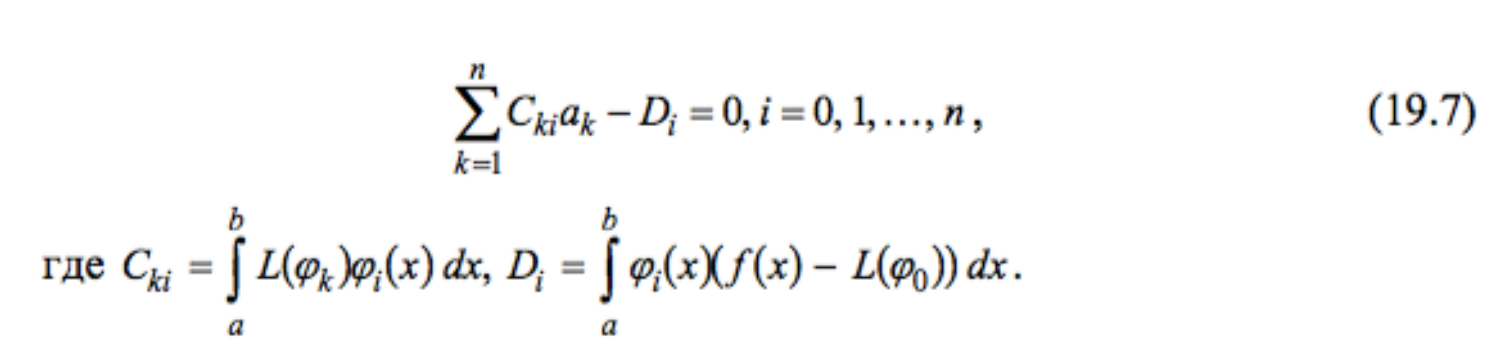
\includegraphics[scale=0.4]{formula1.png}

\begin{enumerate}
    \item Весовые функции
    \begin{enumerate}
        \item $\phi_0 = -1 + x$,
        \item $\phi_1 = (-1 + x) \cdot (2 - x)$,
        \item $\phi_2 = (-1 + x) \cdot (2 - x) ^ 2$.
    \end{enumerate}
    \item Коэффициенты матрицы \begin{equation*}
    A = \begin{pmatrix}
  A_{11} & A_{12} \\
  A_{21} & A_{22} \\
 \end{pmatrix} = \begin{pmatrix}
 -0.3411 & -0.1589\\
 -0.1589 & -0.1351\\
 \end{pmatrix},\end{equation*}
 вектора правой части \begin{equation*}D = \begin{pmatrix}
  D_{1} \\
  D_{2} \\
 \end{pmatrix} = \begin{pmatrix}
  5.864\\
  3.303\\
 \end{pmatrix},\end{equation*} и вектора приближенного решения \begin{equation*}\hat{a} = \begin{pmatrix}
  a_{1} \\
  a_{2} \\
 \end{pmatrix} = \begin{pmatrix}
  -12.84\\
  -9.345\\
 \end{pmatrix},\end{equation*} системы линейных уравнений.
    \item Максимальная глобальная относительная погрешность приближённого $\hat{u} (x)$ и точного $u(x)$  решений — величина
    \begin{equation*}
        \max\limits_{n = \overline{1, N-1}} \left| \dfrac{u(x_n) - \hat{u}(x)}{u(x_n)} \right| = 0.2141,
    \end{equation*}
    \item Графики приближённого $\hat{u}(x)$ и точного $u(x)$ решений на одном рисунке:

    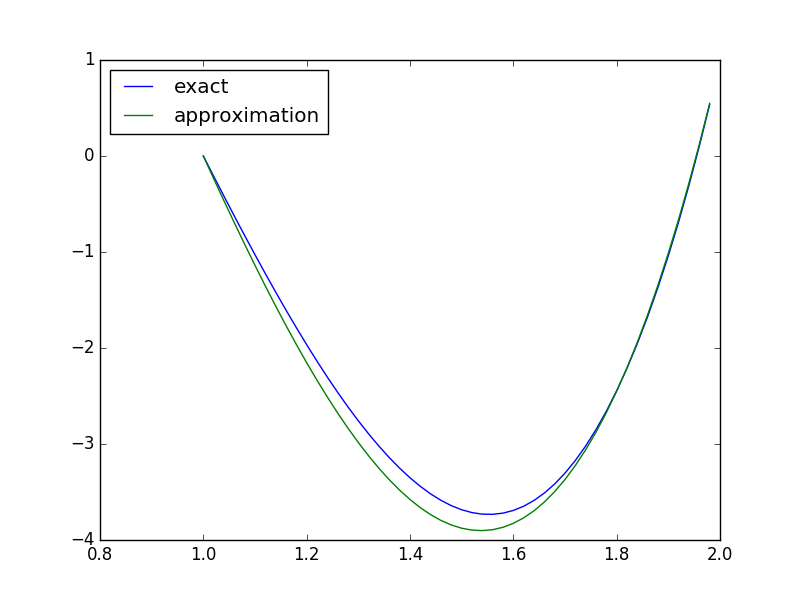
\includegraphics[scale=0.5]{plot1.png}
\end{enumerate}

\lstinputlisting[language=Python, caption=Метод Галёркина, label=lst:code]{galerkin.py}

\subsection{Задание 2}
\begin{enumerate}
    \item Весовые функции:
    \begin{enumerate}
        \item $\phi_0 = -1 + x$,
        \item $\phi_1 = (-1 + x) \cdot (2 - x)$,
        \item $\phi_2 = (-1 + x) \cdot (2 - x) ^ 2$,
        \item $p(x) = 1$,
        \item $q(x) = \dfrac{1}{x}$.
    \end{enumerate}
    \item Коэффициенты матрицы \begin{equation*}
    A = \begin{pmatrix}
  A_{11} & A_{12} \\
  A_{21} & A_{22} \\
 \end{pmatrix} = \begin{pmatrix}
   0.3559 & 0.1774\\
   0.1774 & 0.1393 \\
  \end{pmatrix},\end{equation*}
 вектора правой части \begin{equation*}D = \begin{pmatrix}
  D_{1} \\
  D_{2} \\
 \end{pmatrix} = \begin{pmatrix}
  -5.803\\
  -3.280 \\
 \end{pmatrix},\end{equation*} и вектора приближенного решения \begin{equation*}\hat{a} = \begin{pmatrix}
  a_{1} \\
  a_{2} \\
 \end{pmatrix} = \begin{pmatrix}
  -12.50\\
  -7.631\\
 \end{pmatrix},\end{equation*} системы линейных уравнений.
    \item Максимальная глобальная относительная погрешность приближённого $\hat{u} (x)$ и точного $u(x)$  решений — величина
    \begin{equation*}
        \max\limits_{n = \overline{1, N-1}} \left| \dfrac{u(x_n) - \hat{u}(x)}{u(x_n)} \right| = 0.2711,
    \end{equation*}
    \item Графики приближённого $\hat{u}(x)$ и точного $u(x)$ решений на одном рисунке:

    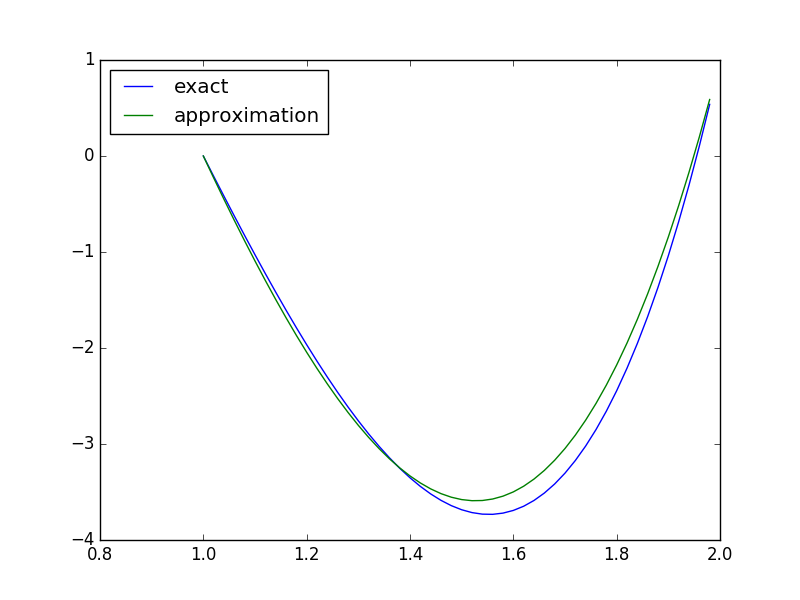
\includegraphics[scale=0.5]{plot2.png}
\end{enumerate}

\lstinputlisting[language=Python, caption=Метод Ритца, label=lst:code]{ritz.py}

\subsection{Задание 3}
Использованые формулы:
\begin{equation*}
    y^{'}_{\alpha} = \dfrac{y_{\alpha}}{x} + 15 x^2,
\end{equation*}
$y_{\alpha}$ - приближение $u^{'}$, которое было найдено с начальным условием \eqref{eq:variant} $y_{\alpha}(1) = \alpha$.
\begin{equation*}
    u^{'}_{\alpha} = y_{\alpha}
\end{equation*}
\begin{equation*}
    \alpha = \alpha - \dfrac{-1 + u_\alpha(2)}{u^{'}_\alpha(2)}
\end{equation*}

\begin{enumerate}
    \item Число итераций метода Ньютона $= 72$.
    \item Абсолютная погрешность второго краевого условия $= 0.04387$.
    \item Максимальная глобальная относительная погрешность
    \begin{equation*}
        \max\limits_{n = \overline{1, N-1}} \left| \dfrac{u(x_n) - \hat{u}(x)}{u(x_n)} \right| = 0.04456.
    \end{equation*}
\end{enumerate}

\lstinputlisting[language=Python, caption=Метод Стрельбы, label=lst:code]{shooting-method.py}
\end{document}
